%===================================================================================
\chapter{Code Organization}\label{s:organization}
%===================================================================================

%----------------------------------
\section{SUNDIALS organization}\label{ss:sun_org}
%----------------------------------
% This is a shared SUNDIALS TEX file with description of
% the SUNDIALS organization
%
The family of solvers referred to as {\sundials} consists of the solvers
{\cvode} (for ODE systems), {\kinsol} (for nonlinear algebraic
systems), and {\ida} (for differential-algebraic systems).  In addition,
{\sundials} also includes variants of {\cvode} and {\ida} with sensitivity analysis 
capabilities (using either forward or adjoint methods): {\cvodes} and {\idas},
respectively.

The various solvers of this family share many subordinate modules.
For this reason, it is organized as a family, with a directory
structure that exploits that sharing (see Fig. \ref{f:sunorg}).
\begin{figure}
\subfigure[High-level diagram]
{\centerline{\psfig{figure=sunorg1.eps,width=\textwidth}}}
\subfigure[Directory structure of the source tree]
{\centerline{\psfig{figure=sunorg2.eps,width=\textwidth}}}
\caption {Organization of the SUNDIALS suite}\label{f:sunorg}
\end{figure}
The following is a list of the solver packages presently available:
\begin{itemize}

\item {\cvode},  
  a solver for stiff and nonstiff ODEs $dy/dt = f(t,y)$;

\item {\cvodes},
  a solver for stiff and nonstiff ODEs
  with sensitivity analysis capabilities;

\item {\ida},
  a solver for differential-algebraic systems $F(t,y,y^\prime) = 0$;

\item {\idas},
  a solver for differential-algebraic systems
  with sensitivity analysis capabilities;

\item {\kinsol}, 
  a solver for nonlinear algebraic systems $F(u) = 0$.

\end{itemize}


%----------------------------------
\section{CVODE organization}\label{ss:cvode_org}
%----------------------------------

\index{CVODE@{\cvode}!package structure}
The {\cvode} package is written in ANSI {\CC}. The following
summarizes the basic structure of the package, although knowledge
of this structure is not necessary for its use.

The overall organization of the {\cvode} package is shown in Figure
\ref{f:cvorg}. 
\begin{figure}[!ht]
{\centerline{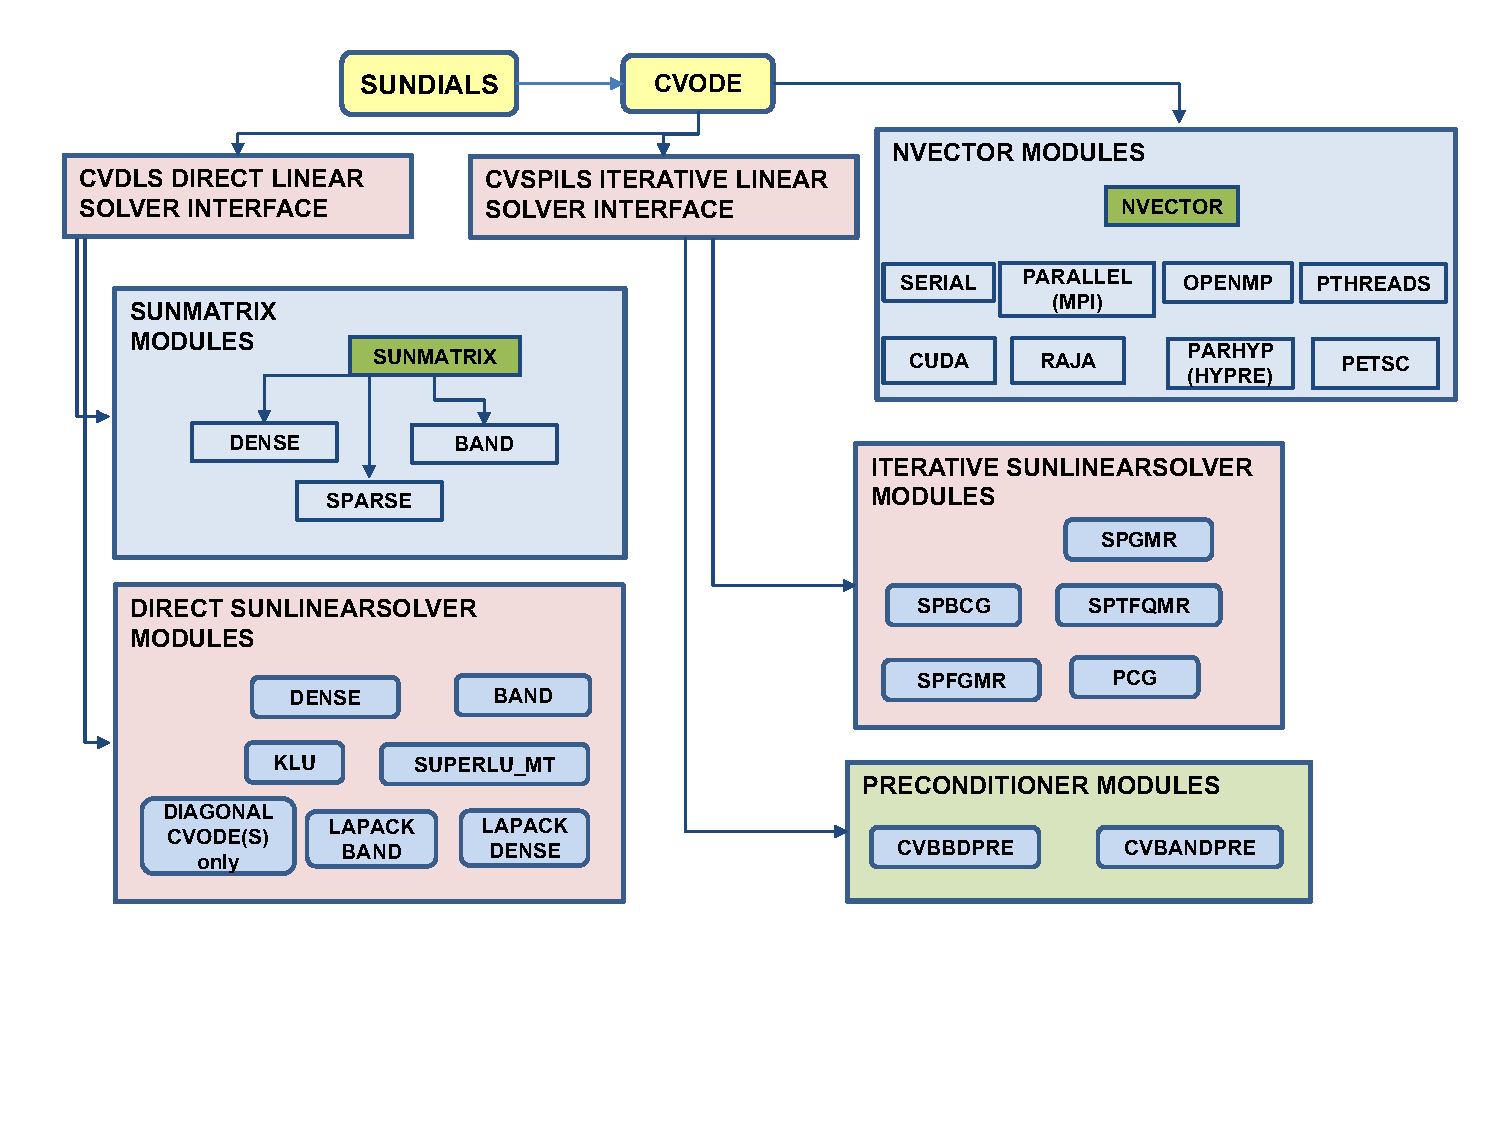
\includegraphics[width=\textwidth]{cvorg}}}
\caption [Overall structure diagram of the {\cvode} package]
{Overall structure diagram of the {\cvode} package.
  Modules specific to {\cvode} begin with ``CV'' ({\cvdls},  {\cvdiag},
  {\cvspils}, {\cvbbdpre} and {\cvbandpre}), all other items correspond
  to generic solver and auxiliary modules. 
  Note also that the LAPACK, {\klu} and {\superlumt} support is
  through interfaces to external packages.  Users will need to
  download and compile those packages independently.}
\label{f:cvorg}
\end{figure}
The central integration module, implemented in the files \id{cvode.h},
\id{cvode\_impl.h}, and \id{cvode.c}, deals with the evaluation of integration
coefficients, the functional or Newton iteration process, estimation of local
error, selection of stepsize and order, and interpolation to user output
points, among other issues.  Although this module contains logic for
the basic Newton iteration algorithm, it has no knowledge of the
method being used to solve the linear systems that arise.  For any
given user problem, one of the linear system solver interfaces is
specified, and is then invoked as needed during the integration. 

\index{CVODE@{\cvode} linear solver interfaces|(} 
At present, the package includes two linear solver interfaces.  The
{\em direct} linear solver interface, {\cvdls}, supports {\sunlinsol}
implementations with type \id{SUNLINSOL\_DIRECT} (see Chapter
\ref{s:sunlinsol}).  These linear solvers utilize direct methods for
the solution of linear systems stored using one of the {\sundials} generic
{\sunmatrix} implementations (dense, banded or sparse; see
Chapter \ref{s:sunmatrix}).  It is assumed that the dominant cost for
such solvers occurs in factorization of the linear system matrix $M$,
so {\cvode} utilizes these solvers within its modified Newton
nonlinear solve. 
The {\em spils} linear solver interface, {\cvspils}, supports
{\sunlinsol} implementations with type \id{SUNLINSOL\_ITERATIVE}
(see Chapter \ref{s:sunlinsol}).  These linear solvers utilize scaled
preconditioned iterative methods.  It is assumed that these methods
are implemented in a ``matrix-free'' manner, wherein only the action
of the matrix-vector product $Mv$ is required.  Since {\cvode} can
operate on any valid {\sunlinsol} implementation of
\id{SUNLINSOL\_DIRECT} or \id{SUNLINSOL\_ITERATIVE} types, the set of
linear solver modules available to {\cvode} will expand as new
{\sunlinsol} modules are developed.

Additionally, {\cvode} includes the {\em diagonal} linear solver
interface, {\cvdiag}, that creates an internally generated diagonal
approximation to the Jacobian.
\index{CVODE@{\cvode} linear solver interfaces|)} 

Within the {\cvdls} interface, the package includes algorithms for the
approximation of dense or banded Jacobians through difference 
quotients, but the user also has the option of supplying the Jacobian
(or an approximation to it) directly.  This user-supplied 
routine is required when using sparse Jacobian matrices, since
standard difference quotient approximations do not leverage the
inherent sparsity of the problem.

Within the {\cvspils} interface, the package includes an algorithm for
the approximation by difference quotients of the product $Mv$. Again,
the user has the option of providing routines for this operation, in
two phases: setup (preprocessing of Jacobian data) and multiplication.
For preconditioned iterative methods, \index{preconditioning!setup and solve phases} 
the preconditioning must be supplied by the user, again in two phases: 
setup and solve.  While\index{preconditioning!advice on} there is no
default choice of preconditioner analogous to the difference-quotient
approximation in the direct case, the references
\cite{BrHi:89,Byr:92}, together with the example and demonstration
programs included with {\cvode}, offer considerable assistance in
building preconditioners. 

\index{CVODE@{\cvode} linear solvers!implementation details|(} 
Each {\cvode} linear solver interface consists of four primary phases,
devoted to (1) memory allocation and initialization, (2) setup of the
matrix data involved, (3) solution of the system, and (4) freeing of memory.  
The setup and solution phases are separate because the evaluation of
Jacobians and preconditioners is done only periodically during the
integration, and only as required to achieve convergence. 
\index{CVODE@{\cvode} linear solvers!implementation details|)} 

{\cvode} also provides two preconditioner modules, for use with any of
the Krylov iterative linear solvers. The first one, {\cvbandpre},
is intended to be used with {\nvecs}, {\nvecopenmp} or {\nvecpthreads}
and provides a banded difference-quotient Jacobian-based
preconditioner, with corresponding setup and solve routines.
The second preconditioner module, {\cvbbdpre}, works in conjunction
with {\nvecp} and generates a preconditioner that is a block-diagonal
matrix with each block being a banded matrix.

All state information used by {\cvode} to solve a given problem is saved
in a structure, and a pointer to that structure is returned to the
user.  There is no global data in the {\cvode} package, and so, in this
respect, it is reentrant. State information specific to the linear
solver is saved in a separate structure, a pointer to which resides in
the {\cvode} memory structure. The reentrancy of {\cvode} was motivated
by the anticipated multicomputer extension, but is also essential
in a uniprocessor setting where two or more problems are solved by
intermixed calls to the package from within a single user program.
